\documentclass[conference]{IEEEtran}
\IEEEoverridecommandlockouts
% The preceding line is only needed to identify funding in the first footnote. If that is unneeded, please comment it out.
\usepackage{cite}
\usepackage{amsmath,amssymb,amsfonts}
\usepackage{algorithmic}
\usepackage{graphicx}
\usepackage{wrapfig}
\usepackage{textcomp}
\usepackage{xcolor}
\def\BibTeX{{\rm B\kern-.05em{\sc i\kern-.025em b}\kern-.08em
    T\kern-.1667em\lower.7ex\hbox{E}\kern-.125emX}}
    
\usepackage[utf8]{inputenc}
\usepackage[spanish]{babel}
\usepackage{lettrine}
\usepackage{fancyhdr}
\pagestyle{fancy}


    
\begin{document}

\fancyhf{} 
\rhead[]{\thepage}
\renewcommand{\footrulewidth}{0.5pt}
\rfoot[]{DPTO. ELECTRÓNICA – CÁTEDRA ELECTRÓNICA DE POTENCIA – 9541- 011/21}

\title{Análisis y Simulación en OrCAD de un Convertidor de Potencia Tipo Ćuk}

\author{\IEEEauthorblockN{Villegas Vidal Sebastián}
\IEEEauthorblockA{\textit{svillegas74@gmail.com}}
\textit{UTN - FRC}}

\maketitle

\begin{abstract} %breve descripción del trabajo%
Los convertidores DC-DC son circuitos que controlan el flujo de energía entre dos sistemas de corriente continua. Se los puede definir como circuitos que controlan la carga y descarga de sus elementos pasivos almacenadores de energía. El convertidor Ćuk no aislado a diferencia de las topologías básicas (Buck, Boost y Buck-Boost), utiliza un capacitor para la transferencia de energía entrada-salida a lo largo del ciclo de conmutación, de tal forma el uso de este capacitor permite obtener una mejor relación entre la energía almacenada y el tamaño del convertidor.

La intención de este trabajo es realizar un análisis completo de esta topología y una simulación del mismo utilizando la herramienta de simulación OrCAD.
\end{abstract}

\def\abstractname{Abstract}

\begin{abstract} %breve descripción del trabajo%
DC-DC converters are circuits that control the flow of power between two DC systems. They can be defined as circuits that control the charging and discharging of their passive energy storage elements. The non-isolated Ćuk converter unlike the basic topologies (Buck, Boost and Buck-Boost), uses a capacitor for the input-output energy transfer along the switching cycle, so the use of this capacitor allows to obtain a better ratio between the stored energy and the size of the converter.

The intention of this work is to perform a complete analysis of this topology and a simulation of it using the OrCAD simulation tool.
\end{abstract}

\begin{IEEEkeywords} %palabras claves%
Converter, Ćuk, Power electronics, OrCad
\end{IEEEkeywords}

\section{Introducción}
\lettrine[lines=2]{E}{L} convertidor de tipo Ćuk, llamado así en honor a su inventor (Slobodan Ćuk), proporcina un voltaje de salida de polaridad negativa respecto al terminal común del voltaje de entrada. La función principal de este convertidor es la de mantener una tensión de salida regulada frente a variaciones en la tensión de entrada o variaciones en la carga. Al igual que con los convertidores de tipo \textit{buck-boost}, el convertidor Ćuk pueden proporcionar un voltaje de salida que puede ser menor o mayor que el voltaje de entrada, sin embargo, la polaridad es opuesta a la del voltaje de entrada. De aquí que se lo conozca también como convertidor inversor.

En la figura \ref{fig: convertidorĆuk} se muestra la topología de este convertidor en configuración no aislada.

\begin{figure}[h]
    \centerline{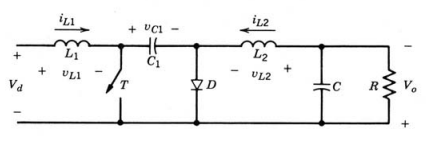
\includegraphics[scale=0.8]{imagenes/convertidor cuk.jpg}}
    \caption{Convertidor Ćuk}
    \label{fig: convertidorĆuk}
\end{figure}

Este convertidor garantiza corriente de entrada continua (ventaja del convertidor boost) y corriente suave en el capacitor de salida (ventaja del convertidor buck). Vale aclarar que el capacitor $C_1$ es el medio para la transferencia de energía desde la fuente hacia la carga.

\section{Análisis de funcionamiento}
Para hacer un análisis completo del funcionamiento de este dispositivo, debemos hacerlo durante los dos modos de conducción a lazo abierto.

Para simplificación del análisis vamos a tener en cuenta las siguientes consideraciones:
\begin{itemize}
    \item El valor de los dos inductores y de los capacitores es grande, las corrientes y tensiones respectivas son constantes (no se producen discontinuidades).
    \item El circuito opera en régimen permanente, por lo que las formas de onda de tensión y corriente son periódicas.
    \item El conmutador y el diodo son ideales.
    \item Resistencias parásitas son insignificantemente pequeñas.
\end{itemize}

\subsection{Modo de conducción continua (CCM)}
\subsubsection{Durante $t_{on}$}
Cuando el interruptor se cierra, como vemos en la figura \ref{fig: Ćuk ton}, fuente de entrada se conecta con el inductor $L_1$, al mismo tiempo, el diodo queda polarizado inversamente, debido a esto la intesidad que circula por $L_1$ crece de forma lineal, almacenando energía. Durante ese mismo instante, el pin positivo de $C_1$ se conecta a masa, polarizando inversamente al diodo. Este capacitor, descarga la energía almacenada a través de $C_2$ y $L_2$, debido a que $V_{C1}>V_o$. Por tanto, se produce un incremento en $i_{L2}$. La entrada alimenta de energía al inductor $L_1$, lo que causa que $i_{L1}$ aumente.

\begin{figure}[h]
    \centering
    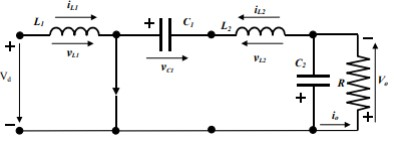
\includegraphics[scale=0.8]{imagenes/cuk ton.jpg}
    \caption{Topología del convertidor Ćuk durante el periodo $T_{on}$}
    \label{fig: Ćuk ton}
\end{figure}

Suponiendo que el voltaje de $C_1$ es contante, se puede equiparar la integral de los voltajes a través de los inductores durante un periodo, resultando en:

\begin{equation}
    V_{L1}=V_d
\end{equation}

Como consecuencia de esto el valor de la variación de corriente circula por los inductores durante $t_{on}$ es:

\begin{equation}
    \Delta I_{L1}=\frac{V_d}{L_1}\cdot t_{on}
    \label{ecu: deltail1}
\end{equation}

Asumimos que la corriente que circula por $L_2$ se incrementa linealmente durante $t_{on}$ debido a la descarga de energía del capacitor de transferencia ($C_1$).
\begin{equation}
    V_{C1}=V_{o}+V_{L2}
\end{equation}

\begin{equation}
    \Delta I_{L2}=\frac{V_{C1}-V_o}{L_2}\cdot t_{on}
\end{equation}

\subsubsection{Durante $t_{off}$}

Transcurrido un tiempo, el interruptor se abre, como es mostrado en la figura \ref{fig: Ćuk toff}. En ese momento el diodo se polariza en directa y la energía almacenada en el inductor $L_1$ junto con la energía de la entrada se transfieren al capacitor $C_1$. Durante éste periodo de tiempo la fuente no entrega ningún tipo de energía a la carga, ocasionando que el inductor $L_2$ entregue su energía almacenada y cuando este se descargue, lo haga capacitor $C_2$.

\begin{figure}[h]
    \centering
    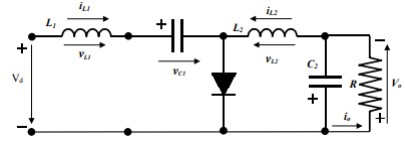
\includegraphics[scale=0.8]{imagenes/cuk toff.jpg}
    \caption{Topología del convertidor Ćuk durante el periodo $T_{off}$}
    \label{fig: Ćuk toff}
\end{figure}

Si analizamos rápidamente mediante LKV tenemos:

\begin{equation}
    V_{L1}=V_d-V_{C1}
\end{equation}

\begin{equation}
    V_{L2}=-Vo
\end{equation}

El valor de la variación de corriente que circula por los inductores durante $t_{off}$ es:

\begin{equation}
    \Delta I_{L1}=\frac{V_d-V_{C1}}{L_1}\cdot t_{off}T
    \label{ecu: deltail1-2}
\end{equation}

Al mismo tiempo, la corriente fluye por el inductor $L_2$, y decrece linealmente.
\begin{equation}
    \Delta I_{L2}=\frac{-V_o}{L_2}\cdot t_{off}T
\end{equation}

\section{Formas de onda del convertidor Ćuk}

\begin{figure}[h!]
    \centering
    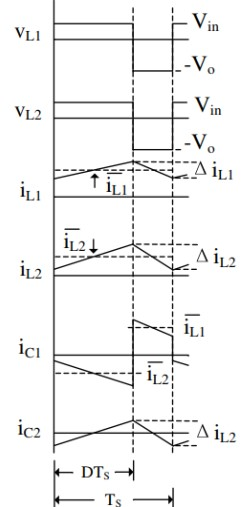
\includegraphics[scale=0.8]{imagenes/forma de onda.jpg}
    \caption{Formas de onda en los diferentes elementos del convertidor Ćuk en CCM}
    \label{fig: forma de odna}
\end{figure}

Una vez obtenidos los valores de la variación de la corriente en cada una de las inductancias y teniendo en cuenta que $\Delta I_L=I_{Lmáx}-I_{Lmín}$ los valores máximos y mínimos de la corriente por los inductores son:
\begin{equation}
    I_{L2máx}=I_{L2}+ \left| \frac{\Delta I_{L2}}{2} \right| 
\end{equation}

\begin{equation}
    I_{L2min}=I_{L2}- \left| \frac{\Delta I_{L2}}{2} \right| 
\end{equation}

\subsection{Modo de conducción discontinua (DCM)}
La salida regulada de tensión en DCM no tiene una relación lineal con la tensión de entrada como
en CCM. Este modo de conducción tiene sus bases en la corriente que pasa a través de los inductores del convertidor especialmente en el inductor $L_2$ (para el inductor $L_1$ el análisis es exactamente similar). Cuando otros convertidores como el Boost o Buck se encuentran en el modo de conducción discontinua sucede que la corriente que pasa por el inductor durante el periodo $t_{off}$ es cero, mientras que en el convertidor Ćuk la corriente por el inductor se puede revertir.

En el DCM se da cuando la inductancia $L_2$ al principio del periodo $t_{off}$ tiene un valor de corriente cero y luego disminuye su valor por debajo de cero hasta que la corriente que pasa por el diodo llega a cero, cuando el diodo vuelve a conducir la corriente que pasa por la inductancia aumenta de nuevo su valor, lo que crea una parte plana por debajo de cero en la corriente de la inductancia conocida como 
$I_{LO}$ como se muestra en la figura \ref{fig: ondas dcm}

\begin{figure}[h!]
    \centering
    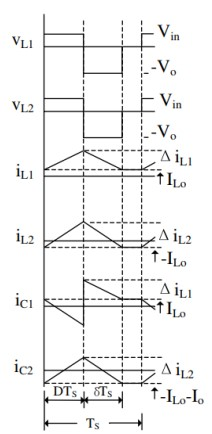
\includegraphics[scale=0.8]{imagenes/dcm.jpg}
    \caption{Formas de onda en los diferentes elementos del convertidor Ćuk en DCM}
    \label{fig: ondas dcm}
\end{figure}

\section{Función de transferencia}
En estado estacionario, la función de transferencia puede ser determinada por la corriente media a través del condensador en un período que debe ser cero. Por lo tanto, mediante la resolución de la ecuación lineal durante el encendido y el apagado, la tensión de salida media se deriva de la siguiente manera. Si suponemos que el voltaje del condensador $V_{C1}$ es constante, equiparar la integral de los voltajes a través de $L_1$ y $L_2$ a lo largo de un periodo resulta en:

Para $L_1$:
\begin{equation}
    V_d\cdot t_{on}+(V_d-V_{C1})\cdot t_{off}=0
\end{equation}

\begin{equation}
    V_{C1}=\frac{V_d}{1-D}
    \label{ecu: vc1-1}
\end{equation}

Para L2:
\begin{equation}
    (V_{C1}-V_o)\cdot t_{on}+(-V_o)\cdot t_{off}=0
\end{equation}

\begin{equation}
    V_{C1}=\frac{V_o}{D}
    \label{ecu: vc1-2}
\end{equation}

Igualando las ecuaciones (\ref{ecu: vc1-1}) y (\ref{ecu: vc1-2}) obtenemos:
\begin{equation}
    \frac{V_d}{1-D}=\frac{V_o}{D}
\end{equation}

Obtenemos finalmente:

\begin{equation}
    \frac{V_o}{V_d}=\frac{D}{1-D}
    \label{ecu: fcn trans}
\end{equation}


\section{DETERMINACIÓN DE COMPONENTES}
El análisis realizado hasta ahora nos sirve para seleccionar los componentes necesarios para garantizar que el convertidor opere en CCM. En el análisis anterior, el condensador $C_2$ se supone que es muy grande para mantener constante la tensión de salida. En la práctica, la tensión de salida no puede mantenerse perfectamente constante con una capacitancia finita. La variación en la tensión de salida, o la ondulación, es calculada a partir de la relación de tensión de corriente del condensador.

Si consideramos el periodo de tiempo de conmutación:
\begin{equation}
    T=\frac{1}{f_s}=t_{on}+t_{off}
\end{equation}

Podemos despejar $t_{on}$ y $t_{off}$ de las ecuaciones (\ref{ecu: deltail1}) y (\ref{ecu: deltail1-2})
\begin{equation}
    =\frac{L_1\Delta I_{L1}}{V_d}+\frac{L_1\Delta I_{L1}}{V_d-V_{C1}}
\end{equation}

\begin{equation}
    =\frac{L_1\Delta I_{L1}}{V_d D}
\end{equation}

\begin{equation}
    L_1=\frac{V_d\cdot D}{f_s\Delta I_{L1}}
\end{equation}

Analizando la ecuación de salida de la misma forma:
\begin{equation}
    L_2=\frac{V_d\cdot D}{f_s\Delta I_{L2}}
\end{equation}

Para que la corriente sea continua en las bobinas, la corriente media debe ser mayor que la mitad del cambio en la corriente. Sus valores lo podemos calcular mediante:
\begin{equation}
    L_{1min}=\frac{(1-D)^2\cdot R}{2Df}    
\end{equation}

\begin{equation}
    L_{2min}=\frac{(1-D)\cdot R}{2\cdot f}
\end{equation}

El voltaje medio a través de $C_2$ se calcula a partir de la LKV. El voltaje medio a través de los indcutores es cero para la operación en estado estacionario, lo que resulta en:

\begin{equation}
    v_{C2}= v_o
\end{equation}

Mientras que la corriente de $C_2$ sea positiva, el capacitor se estará cargando. De la definición de capacidad:

\begin{equation}
    Q=C_2V_o
\end{equation}

\begin{equation}
    \Delta Q=C_2\Delta V_o
\end{equation}

\begin{equation}
    \Delta V_o=\frac{\Delta Q}{C_2}
\end{equation}

El cambio en la carga $\Delta Q$ es el área del triángulo por encima del eje del tiempo, como se muestra en la figura \ref{fig: robo}.

\begin{figure}[h!]
    \centering
    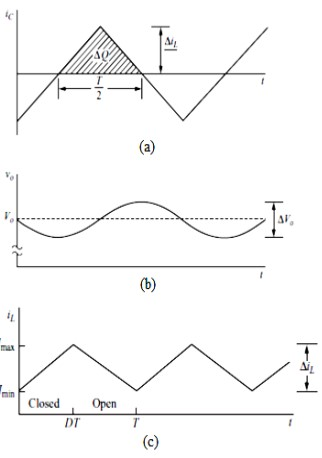
\includegraphics[scale=0.8]{imagenes/robodelsiglo.jpg}
    \caption{(a) la corriente de $C_2$ (b) tensión de rizado en $C_2$ (c) Rizado en $L_2$}
    \label{fig: robo}
\end{figure}

Recordemos que durante el $t_{off}$ el capacitor $C_1$ se carga a través de $L_1$ y la fuente de entrada. La corriente de carga decrece entre los valores picos y de valle de $I_{L2}$, por esto, la corriente promedio de carga es igual a la corriente de entrada. Los productos tiempo corriente de carga y descarga del capacitor de transferencia de energía $C_1$ deberan ser por tanto iguales. Entonces el rizado en $C_1$ se puede estimar calculando el cambio $V_{C1}$ en el intervalo cuando el interruptor esta abierto (y las corrientes $I_{L1}$ y $I_{C1}$ son las mismas). Suponiendo que la corriente en $L_1$ sea constante.

\begin{equation}
    \Delta v_{c1}= \frac{1}{C_1} \int_{0}^{T} i_{L1} \cdot dt=\frac{I_{L1}}{C_1}(1-D)T
\end{equation}

Como $I_{L1}=I_{in}$, podemos reemplzarlo de tal forma que:

\begin{equation}
     \Delta v_{c1}=\frac{I_{in}(1-D)}{C_1f}
\end{equation}

\begin{equation}
    C_1 =\frac{I_{in}(1-D)}{\Delta v_{c1}f}
\end{equation}

Si $\Delta I_{L2}=\Delta I_{C2}$, la corriente de carga promedio del capacitor de salida fluye en un instante $\frac{T}{2}$:

\begin{equation}
    I_{C2}=\frac{\Delta I_{L2}}{4}
\end{equation}

Por tanto:
\begin{equation}
    \Delta v_{c2}= \frac{1}{C_2} \int_{0}^{T/2} i_{L2} \cdot dt=\frac{T\cdot \Delta I_{L2}}{8C_2}
\end{equation}

En esta ecuación. $\Delta V_o$ es el voltaje de ondulación pico a pico en la salida, como se muestra en la figura \ref{fig: robo}-b. El rizado de la tensión de salida es la ondulación de la tensión del capacitor $C_2$.

\begin{equation}
     \Delta v_{c2}=\frac{\Delta I_{L2}}{8fC_2}
\end{equation}

\begin{equation}
    C_2=\frac{\Delta I_{L2}}{8f\Delta v_{c2}}
\end{equation}

Para determinar el ciclo útil de trabajo de nuestro convertidor resulta:
\begin{equation}
    \frac{v_o}{v_d}=\frac{D}{1-D}
\end{equation}

Por lo tanto D:

\begin{equation}
    D=\frac{v_o}{v_d+v_o}
\end{equation}

Para el diodo, se tiene en cuenta la corriente máxima que pasa por él y que su tiempo de conmutación sea rápido. La corriente máxima que pasa por el diodo es la suma de la corriente de entrada ($I_{L1}$) y la corriente de salida ($I_{L2}$)

\begin{equation}
    I_{Dmax}=I_{L1}+I_{L2}
\end{equation}

Para el cálculo del MOSFET se analiza nuevamente cual es la máxima variación en la corriente de entrada y en la corriente de salida que pasa por este dispositivo (estas variaciones se relacionan directamente con el rizado escogido tanto para la inductancia L1 como para la inductancia L2, pues por ambas pasa la corriente de entrada y salida, respectivamente) . 

\begin{equation}
    I_{MOSFET}=\Delta I_{L1}+\Delta I_{L2}
\end{equation}

En la elección de un MOSFET, resulta muy importante realizar un análisis de potencia, pues se deben tener en cuenta tanto la potencia para el periodo de conmutación como la potencia en el periodo de conducción. Lo anterior se relaciona directamente con el valor de voltaje y corriente necesarios para asegurar que el MOSFET entre en la región de saturación sin un consumo de potencia desmesurado. Mediante el cálculo de potencia en el MOSFET es posible aproximar las pérdidas en el periodo de conducción y conmutación por mínimas que sean.

\begin{equation}
    P_{MOSFET}=V_{DS}\cdot I_{DS}\cdot (t_{on}+t_{off})\cdot f
\end{equation}

Asi para $t_{on}$

\begin{equation}
    P_{ton}=V_{DS}\cdot I_{DS}\cdot t_{on}\cdot f
\end{equation}

Y para $t_{off}$:

\begin{equation}
    P_{toff}=V_{DS}\cdot I_{DS}\cdot t_{off}\cdot f
\end{equation}

También es necesario tener en cuenta la potencia de conducción, la cual se expresa:
\begin{equation}
    P_{conduccion}=I_{max}^2\cdot R_{ds(on)}
\end{equation}

La potencia total disipada será:
\begin{equation}
    P_{Total}=P_{ton}+P_{toff}+P_{conduccion}
\end{equation}

\section{CONVERTIDOR TIPO Ćuk AISLADO}
\begin{figure}[h!]
    \centering
    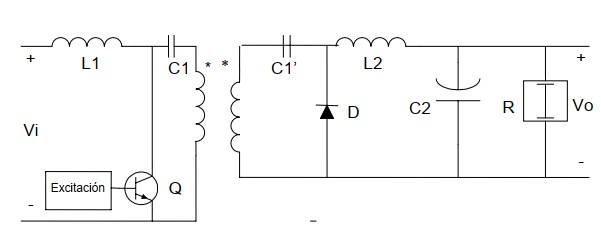
\includegraphics[scale=0.55]{imagenes/aislado.jpg}
    \caption{Circuito de un convertidor Ćuk aislado}
    \label{fig: Ćuk aislado}
\end{figure}

Este circuito, lo podemos ver figura \ref{fig: Ćuk aislado}, opera en forma equivalente al convertidor de Ćuk básico, con el capacitor $C_1$ dividido en dos, uno en serie con la entrada y otro con la salida. La presencia de estos capacitores, al encontrarse en serie con los arrollamientos primario y secundario, previene la existencia de corrientes continuas que puedan producir la saturación del núcleo.

Si el transformador se encuentra magnéticamente acoplado a las dos inductancias, es teóricamente posible ajustar a cero el ripple de las corrientes de entrada y salida.

\section{SIMULACIÓN}
El circuito que usaremos para simular es el de la figura \ref{fig: Ćuk simulado}, para el cual se establecen las siguientes condiciones de diseño:
\begin{itemize}
    \item $\Delta i_{L2}=\Delta i_{L1}=20\%$
    \item $\Delta v_{C1}=5\%$
    \item $\Delta v_{C2}=2\%$ (para una señal con el menor ripple posible)
    \item $f_s=100kHz$
    \item $V_{d}=15V$
    \item $V_o=-30V$
    \item $R=8\Omega$
\end{itemize}

\begin{figure}[h!]
    \centering
    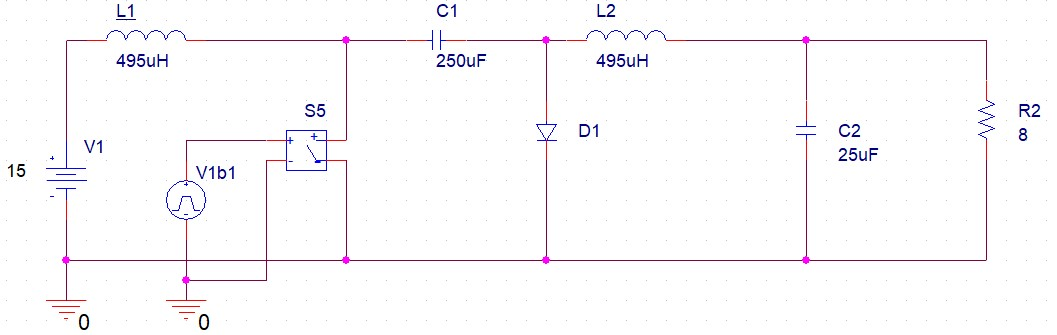
\includegraphics[scale=0.3]{imagenes/cuk-simulado.jpg}
    \caption{Circuito de un convertidor Ćuk simulado}
    \label{fig: Ćuk simulado}
\end{figure}

Los resultados obtenidos para un $D=66\%$ fueron:

\begin{figure}[h!]
    \centering
    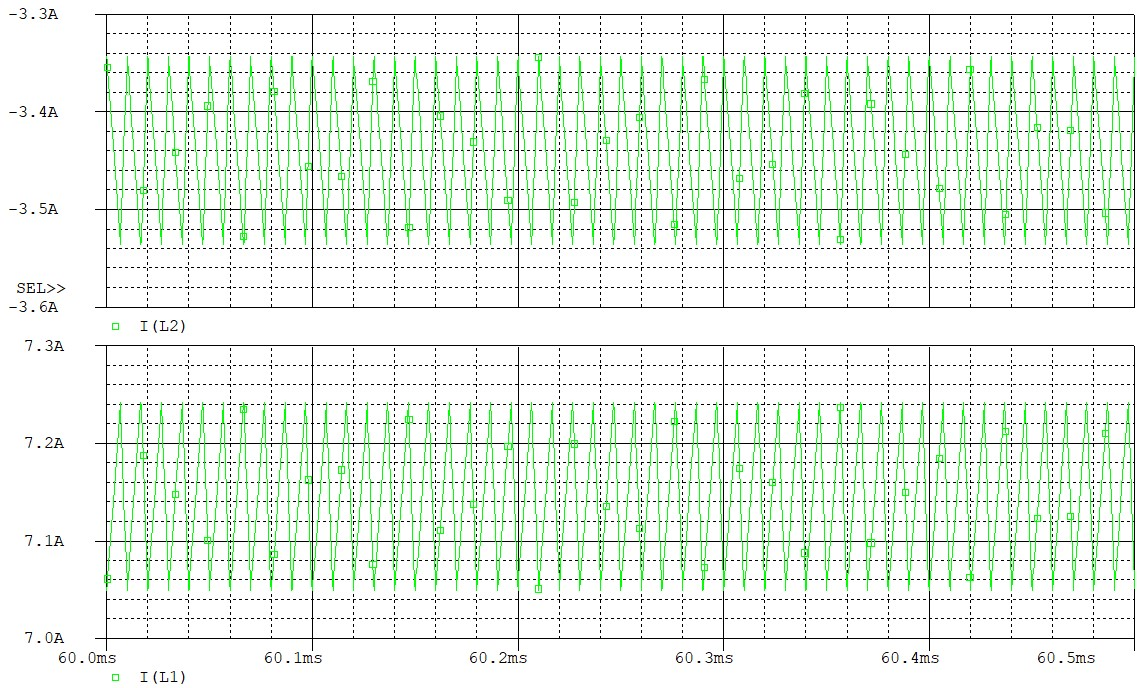
\includegraphics[scale=0.30]{imagenes/il1-il2.jpg}
    \caption{Corriente a través de los inductores L1 y L2}
    \label{fig: il1-il2}
\end{figure}

A primera vista, en la figura \ref{fig: il1-il2} podemos apreciar tanto que el rizado en $L_1$ como $L_2$ es bastante pequeño.

\begin{figure}[h!]
    \centering
    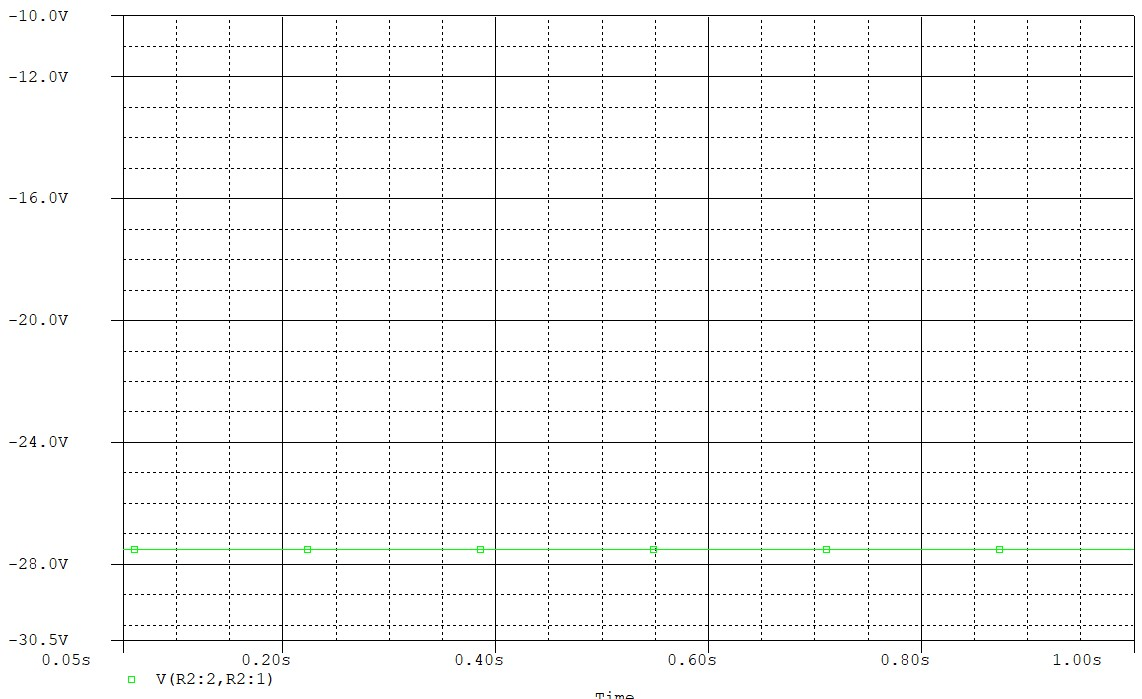
\includegraphics[scale=0.29]{imagenes/vo.jpg}
    \caption{Voltaje de salida $V_o$}
    \label{fig: vo}
\end{figure}

\begin{figure}[h!]
    \centering
    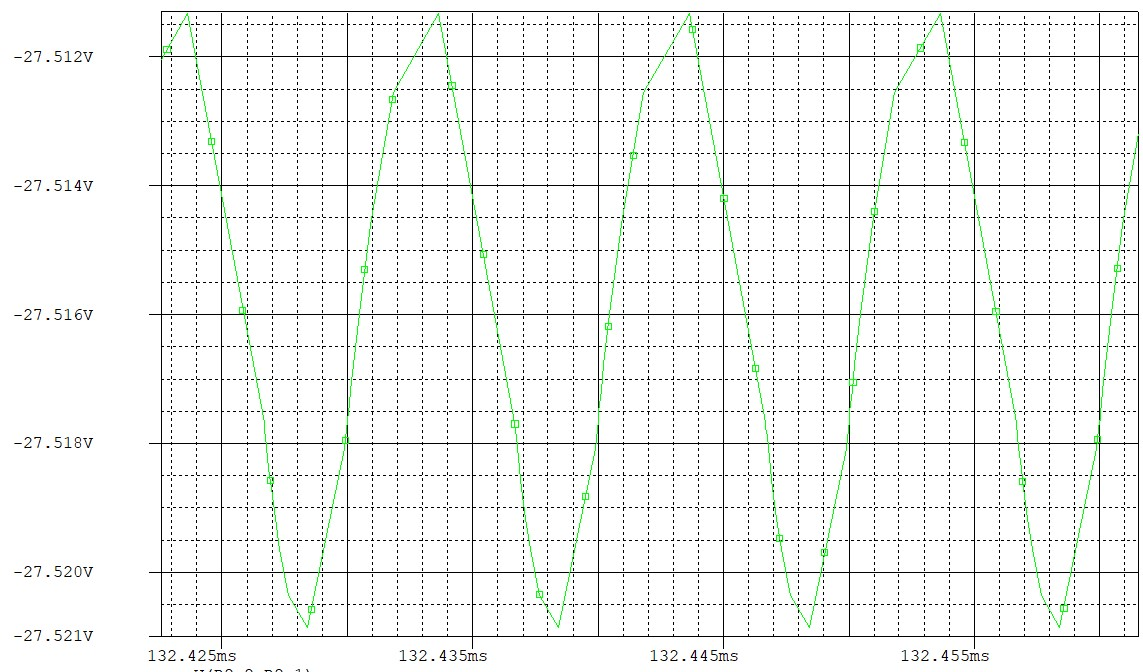
\includegraphics[scale=0.29]{imagenes/vo-rizado.jpg}
    \caption{Ripple de $V_o$}
    \label{fig: vo-rizado}
\end{figure}

En la figura \ref{fig: vo} se aprecia que el voltaje de salida final obtenido fue de aproximadamente $-27,5V$. En la figura \ref{fig: vo-rizado} se aprecia con mayor detenimiento $\Delta v_o$, que tiene un valor aproximado de $-10mV$. En tanto en la figura \ref{fig: vc2}, vemos que se trata del mismo voltaje.

\begin{figure}[h!]
    \centering
    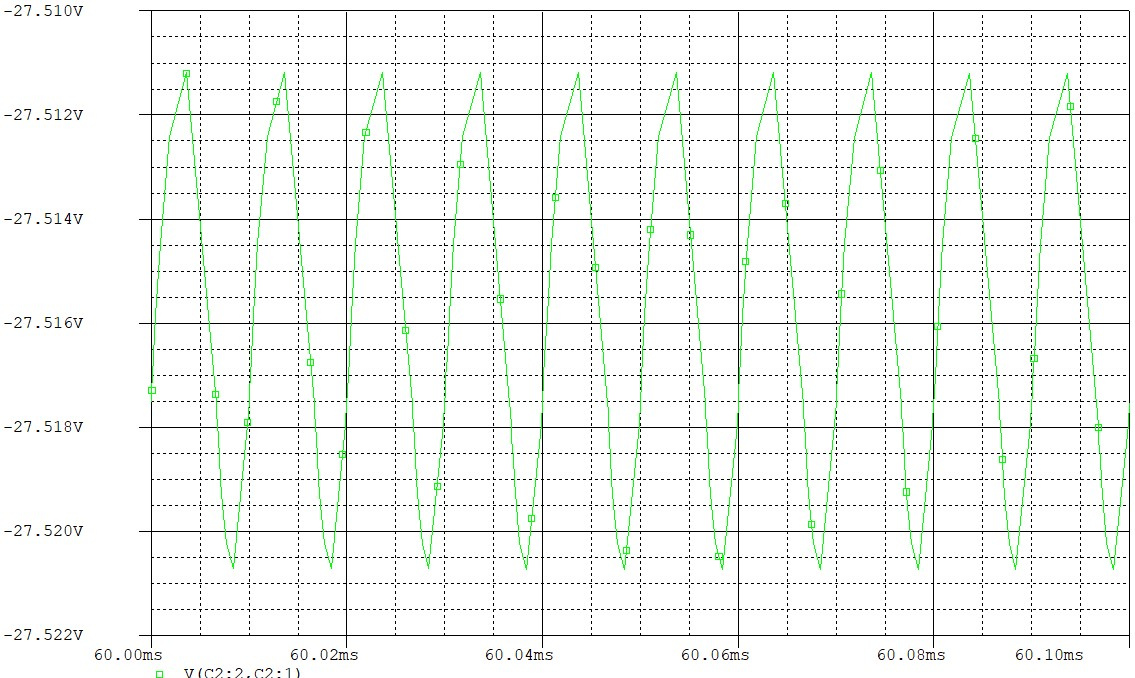
\includegraphics[scale=0.29]{imagenes/vc2.jpg}
    \caption{Voltaje a traves de $V_{C2}$}
    \label{fig: vc2}
\end{figure}

En tanto, el voltaje en el capacitor de transferencia de energía ($C1$) se puede analizar en la figura \ref{fig: vc1}

\begin{figure}[h!]
    \centering
    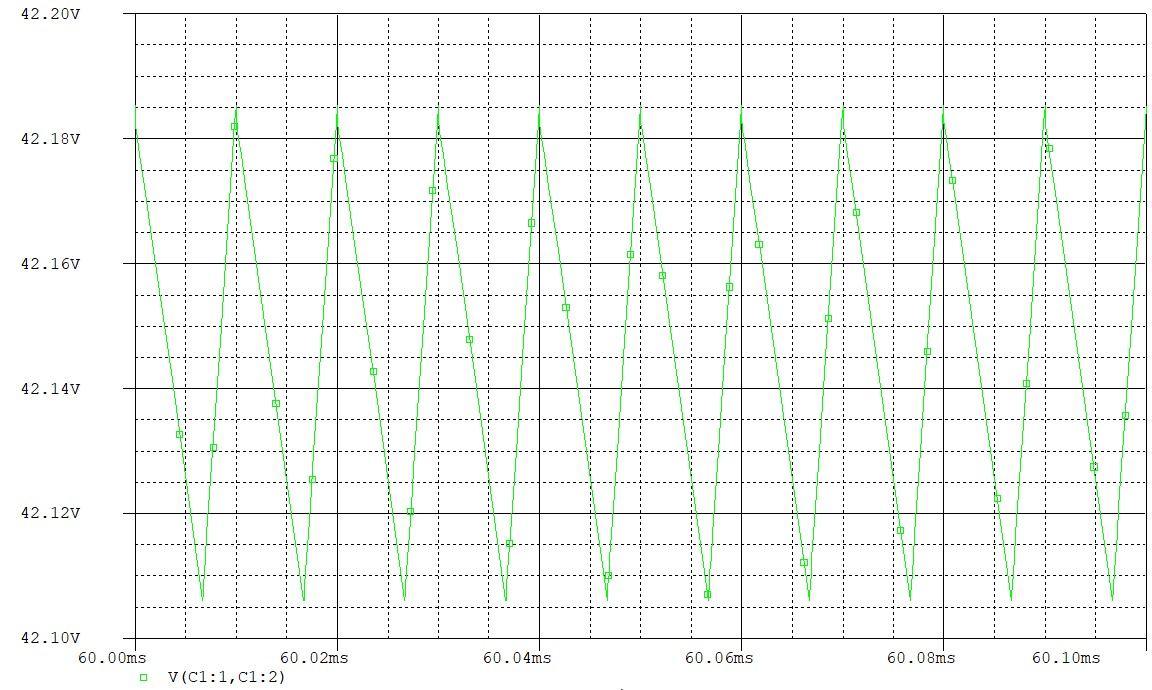
\includegraphics[scale=0.29]{imagenes/vc1.jpg}
    \caption{Voltaje a traves de $V_{C1}$}
    \label{fig: vc1}
\end{figure}

Podemos como se cumple entonces la condición de que $V_{C1}=V_d+V_o$


\section{CONCLUSIONES}
Como vimos con la simulación, la corriente de entrada como así la corriente de salida presentan un bajo ripple de entrada, lo cual forma parte de las grande ventajas de este convertidor. Usualmente en la práctica, los inductores suelen ser montados sobre el mismo núcleo (inductores acoplados), para simplificar un poco su construcción y reducir más el ripple de salida. Además esta clase de convertidor presenta buenos resultados frente a EMI-EMC, tanto la entrada como la salida se encuentran filtradas. Este convertidor además suele presentar una buena eficiencia, debido a que el capacitor de transferencia de energía se descargan a través de inductores, minimizado los picos de corrientes que se puedan producir.

La principal desventaja de este convertidor, es la alta dependencia del capacitor de transferencia de energía, ya que debe soportar toda la potencia exigida al circuito, limitando así a este convertidor en aplicaciones de potencia considerable. El circuito de control debe ser lo bastante preciso como para asegurar el correcto funcionamiento del convertidor, lo cual suele presentar un desafío, debido a los cuatros elementos almacenadores de energía presentes en esta topología.


Gracias al software de simulación OrCad se pudo obtener los valores más relevantes del convertidor en lazo abierto, sin duda, un análisis complementario podría ser aplicando la \textit{Teoría del Control}, para obtener resultados más óptimos y más cercanos a la realidad de aplicación de estos dispositivos.
\\
\begin{thebibliography}{00}
    \bibitem{b1} R.C. Oros, "Fuentes conmutadas" 
\bibitem{b2} Mohan, Ned, "First Course on Power Electronics and Drives" (2003)
\bibitem{b3} Rashid, Muhammad, "Power Electronics", Tercera edición (2004)
\bibitem{b4} Mohan, Ned,Undeland, Tore, Robbins, William, "Electrónica de Potencia-convertidores, aplicaciones y diseño" 
\bibitem{b5} S.C. Garzón Muñoz,  'Análisis de convertidores de potencia DC-DC con
software libre openmodelica', (2012)
\bibitem{b6} A.F. Cifuentes Tobón "Modelo y construcción de un convertidor DC/DC tipo
Cuk para estudio en el laboratorio" (2019)
\bibitem{b7} A. Nachez 'Electrónica de Potencia - Aplicaciones de la conversión CC-CC - Convertidor de Cuk' (2004)
\bibitem{b8} F. Juárez León, E. Rodríguez Segura, "Análisis, diesño e implementación de un convertidor Cuk para iluminación LED"
\bibitem{b9} S. Ang, A. Oliva, "Power-Switching Converters", Segunda edición (2004)
\end{thebibliography}

\section{DATOS BIOGRÁFICOS}
\begin{wrapfigure}{l}{0.25\textwidth} %this figure will be at the right
    \centering
    
\includegraphics[width=0.25\textwidth]{imagenes/foto paper.jpg}
\end{wrapfigure}

\textbf{Sebastián Villegas Vidal}, nacido en Río Gallegos el 25/02/1996. Estudiante de Ingeniería Electrónica, Universidad Tecnológica Nacional, Facultad Regional Córdoba, Argentina. Cursó sus estudios secundarios en el colegio Industrial N° 4 "José Menendez" de su localidad natal, egresando en el año 2014 con el titulo de "Técnico en Electrónica". Inició sus estudios en la Facultad Regional Córdoba de la UTN en la carrera Tecnicatura Superior en Mecatrónica en el año 2015, finalizando la misma en el 2018. Desde el año 2016 que es estudiante de la carrera de grado de Ingeniería Electrónica. 
Sus intereses son: Procesamiento de señales, desarrollo de software en tiempo real, IoT y la róbotica en general.

e-mail: 73643@electronica.frc.utn.edu.ar



\end{document}
